\documentclass[11pt,a4paper]{article}

\usepackage{pifont}
\usepackage{amsmath}
\usepackage{amssymb}
\usepackage{psfig}
\usepackage{graphicx}
\usepackage{array}
\usepackage{fancyheadings}
\usepackage{here}
\usepackage{eepic,epic}
\usepackage[english]{babel}

\input{YRpersdf}

\oddsidemargin -0.9cm
\evensidemargin -0.9cm
\topmargin -1cm
\textheight 22.5cm
\textwidth 17.6cm
\headheight 1.0cm

% principal notations



\begin{document}

\begin{center}
  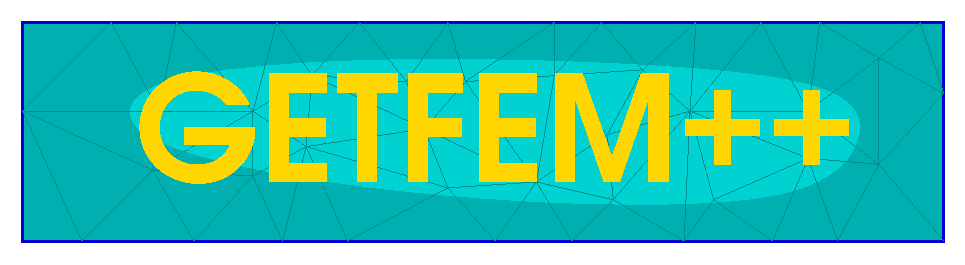
\includegraphics[width=10cm,angle=0]{getfem_logo.eps}\\[0.2cm]
  a Generic Finite Element library in C++ \\[0.5cm]
  {\Huge \sc Short User Documentation} \\[0.5cm]
  { \large Yves \sc Renard\footnote{ \it MIP, INSAT, Complexe scientifique de Rangueil, 31077 Toulouse, France, Yves.Renard@gmm.insa-tlse.fr } } \\[1.0cm]
\end{center}

% \begin{abstract}
% Basic user documentation for GETFEM++.
% \end{abstract}


%%%%%%%%%%%%%%%%%%%%%%%%%%%%%%%%%%%%%%%%%%%%%%%%%%%%%%%%%%%%%%%%%%%%%%%%%
%          INTRODUCTION                                                 %
%%%%%%%%%%%%%%%%%%%%%%%%%%%%%%%%%%%%%%%%%%%%%%%%%%%%%%%%%%%%%%%%%%%%%%%%%

\section*{Introduction}


The GETFEM++ project is centred around the development of a generic and efficient C++ library for elementary computations for finite element methods. The goal is to build a library which allows to compute any elementary matrix (even for mixed methods) on the largest class of methods and elements and for arbitrary dimension. It offers a complete separation between integration methods (exact or approximated), geometric transformations (linear or not) and finite element methods of arbitray degrees.

 Moreover, the library includes other tools for computation with finite element such as assembling methods for classical PDEs, interpolation methods, computation of norms, mesh operations, boundary conditions ... This library allows t build finite elements codes which are completely independent of the dimension, the particular method or element. Examples are provided.\\[5cm]
Copyright (C) 2002\\
The program GETFEM++ is free software; you can redistribute it and/or modify
it under the terms of the GNU General Public License as published by
the Free Software Foundation; version 2 of the License.
This program is distributed in the hope that it will be useful,
but WITHOUT ANY WARRANTY; without even the implied warranty of
MERCHANTABILITY or FITNESS FOR A PARTICULAR PURPOSE.  See the
GNU General Public License for more details.
You should have received a copy of the GNU General Public License
along with this program; if not, write to the Free Software Foundation,
Inc., 59 Temple Place - Suite 330, Boston, MA  02111-1307, USA.

\newpage
\tableofcontents
\newpage

\section{Build a mesh}
GETFEM++ has it own structure to store meshes. This structure is mainly defined in the files {\tt bgeot\_mesh\_structure.h}, {\tt bgeot\_mesh.h} and {\tt getfem\_mesh.h}. The main structure is defined in {\tt getfem\_mesh.h} by the object\\[0.5cm]
{\tt getfem::getfem\_mesh }\\[0.5cm]
This object is able to store any element in any dimension even if you mix elements with different dimensions.\\[0.5cm]

There is no meshing procedures in GETFEM++ to mesh complex geometries. This is no the goal of this package. But you can easily load a mesh from any format.

\subsection{Add an element to a mesh}
Suppose the variable mesh has been declared by\\[0.5cm]
{\tt getfem::getfem\_mesh mesh;}\\[0.5cm]
the you have two way to insert a new element to this mesh : with a list of points or with a list of indexes of already existing points.\\[0.5cm]
One enter a new point on a mesh with the method\\[0.5cm]
{\tt i = mesh.add\_point(pt);}[0.5cm]
where {\tt pt} is of type {\tt bgeot::base\_node}. The index {\tt i} is the index of this point on the mesh. If the point already exists in the mesh, a new point is not inserted and the index of the already existing point is returned. A mesh has a principal dimension, which is the dimension of its points. It is not possible to have points of different dimensions in a same mesh.\\[0.5cm]
The more basic function to add a new element to a mesh is\\[0.5cm]
{\tt j = mesh.add\_convex(pgt, it);}
This is a template function, with {\tt pgt} of type {\tt bgeot::pgeometric\_trans} and {\tt it} is an iterator on a list of indexes of already existing points. For instance, if one needs to add a new triangle in a 3D mesh, one needs to define first an array with the indexes of the three points:\\[0.5cm]
{\tt 
  std::vector<bgeot::size\_type> ind(3); \\
  ind[0] = mesh.add\_point(bgeot::base\_node(0.0, 0.0, 0.0);\\
  ind[1] = mesh.add\_point(bgeot::base\_node(0.0, 1.0, 0.0);\\
  ind[2] = mesh.add\_point(bgeot::base\_node(0.0, 0.0, 1.0);
}\\[0.5cm]
then adding the element is done by
{\tt mesh.add\_convex(bgeot::simplex\_trans(2,1), ind.begin()); }\\[0.5cm]
where {\tt mesh.add\_convex(bgeot::simplex\_trans(N,1);} denotes the usual linear geometric transformation for simplexes of dimension N.\\[0.5cm]
For simplexes, a more specialized function exists, which is\\[0.5cm]
{\tt mesh.add\_simplex(2, ind.begin()); }\\[0.5cm]

It is also possible to give directly the list of points with the function\\[0.5cm]
{\tt mesh.add\_convex\_by\_points(pgt, itp); }\\[0.5cm]
where this time {\tt itp} is an iterator on an array of points. For example\\[0.5cm]
{\tt
  std::vector<bgeot::base\_node> pts(3); \\
  pts[0] = bgeot::base\_node(0.0, 0.0, 0.0); \\
  pts[0] = bgeot::base\_node(0.0, 1.0, 0.0); \\
  pts[0] = bgeot::base\_node(0.0, 0.0, 1.0); \\
  mesh.add\_convex\_by\_points(bgeot::simplex\_trans(2,1), pts.begin());
}\\[0.5cm]
It is possible to use also \\[0.5cm]
{\tt mesh.add\_simplex\_by\_points(2, pts.begin()); } \\[0.5cm]

For other elements than simplexes, it is still possible to use {\tt mesh.add\_convex\_by\_points} or {\tt mesh.add\_convex} with the appropriate geometric transformation. \\[0.5cm]
{\tt bgeot::parallelepiped\_trans(N, 1) }
describes the usual transformation for parallelepipeds of dimension {\tt N} (quadrilateron for {\tt N=2}, hexahedron for {\tt N=3}, ...) \\[0.5cm]
{\tt bgeot::prism\_trans(N, 1) } 
describes the usual transformation for prisms of dimension {\tt N} (usual prism is for {\tt N=3}. A generalized prism is the product of a simplex of dimension {\tt N-1} with a segment) \\[0.5cm]
Specialized functions exist also: \\[0.5cm]
{\tt 
  mesh.add\_parallelepiped(N, it); \\
  mesh.add\_parallelepiped\_by\_points(N, itp); \\
  mesh.add\_prism(N, it); \\
  mesh.add\_prism\_by\_points(N, itp);
} \\[0.5cm]

The order of the points in the array of point is not important for simplexes. For other element, it is important to respect the order shown in figure \ref{fig:elem}.

\begin{figure}[htb] \label{fig:elem}
  \begin{center}
    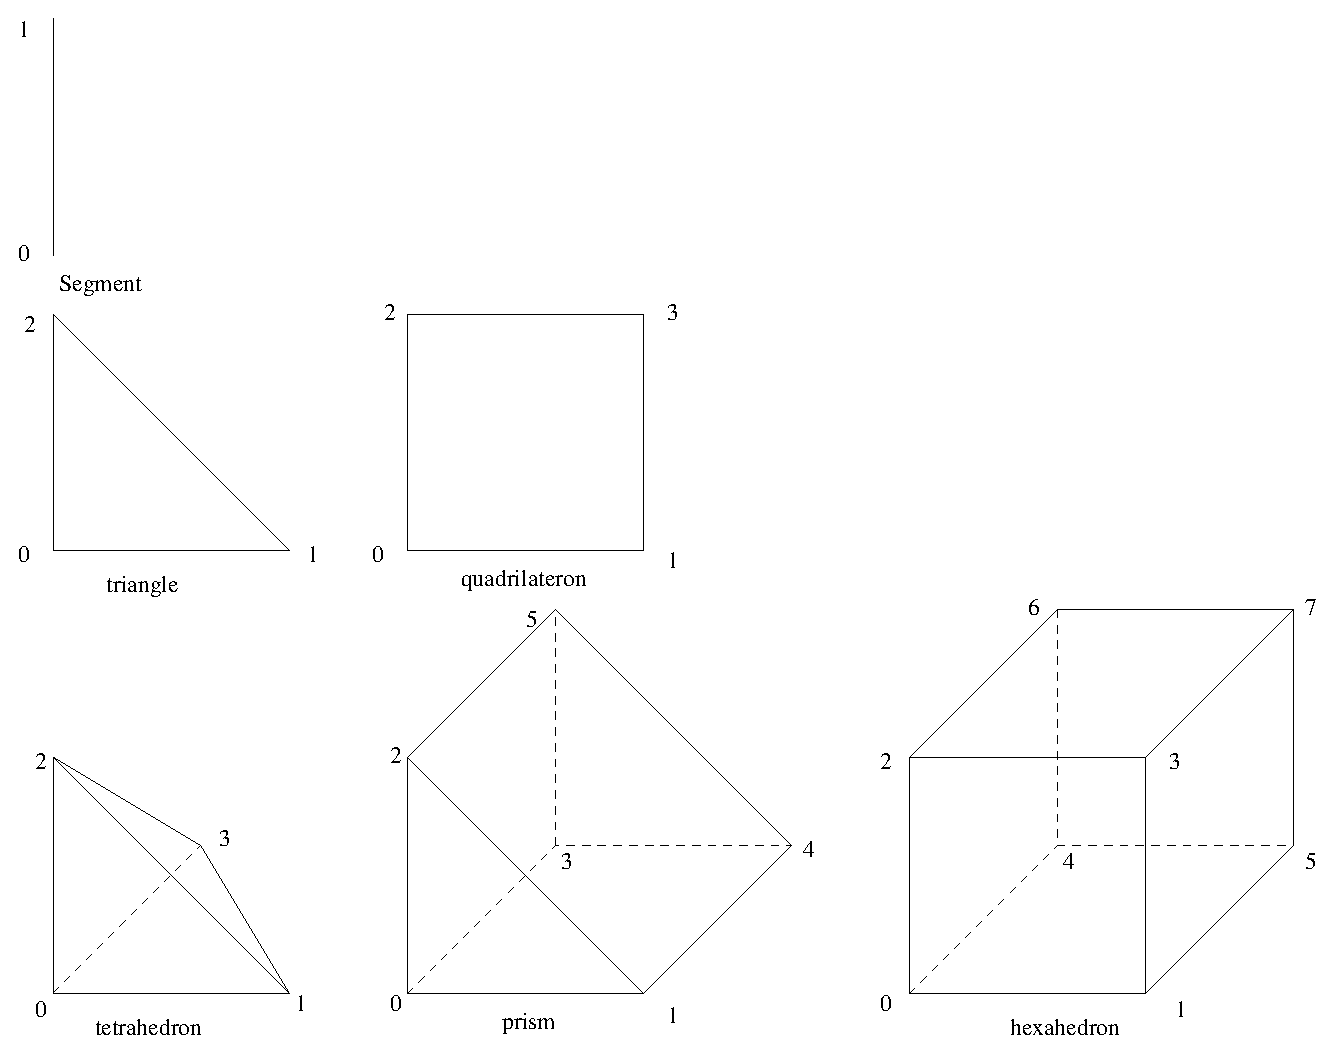
\includegraphics[width=15cm,angle=0]{getfemuser_elem.eps}
  \end{center}
  \caption{ \it vertex numerotation for usual elements }
\end{figure}

\subsection{Remove an element from a mesh}
To remove an element from a mesh, simply use\\[0.5cm]
{\tt mesh.sup\_convex(i); }\\[0.5cm]
where {\tt i} is the index of the element.

\subsection{Simple meshes}

For parallelepiped domains, it is possible to obtain structured meshes with simplexes, parallelepiped or prism element from three functions defined in {\tt getfem\_regular\_meshes.h}. \\[0.5cm]
{\tt
  getfem::parallelepiped\_regular\_simplex\_mesh(mesh, N, org, ivect, iref); \\
  getfem::parallelepiped\_regular\_prism\_mesh(mesh, N, org, ivect, iref); \\
  getfem::parallelepiped\_regular\_mesh(mesh, N, org, ivect, iref);
} \\[0.5cm]
where {\tt mesh} is a mesh variable in which the structured mesh will be built, {\tt N} is the dimension (limited to 4 for simplexes, 5 for prisms, unlimited for parallelepiped), {\tt org} is of type {\tt bgeot::base\_node} and represents the origine of the mesh, {\tt ivect} is an iterator on an array of {\tt N} vectors to build the parallelepiped domain, {\tt iref} is an iterator on an array of {\tt N} integers representing the number of division on each direction. \\[0.5cm]
For instance, to build a mesh with tetrahedrons for a unit cube with $10\times10\times10$ cells one can write\\[0.5cm]
{\tt
  getfem::getfem\_mesh mesh; \\
  bgeot::base\_node org(0.0, 0.0, 0.0); \\
  std::vector<bgeot::base\_vector> vect(3); \\
  vect[0] = bgeot::base\_vector(1.0, 0.0, 0.0); \\
  vect[1] = bgeot::base\_vector(0.0, 1.0, 0.0); \\
  vect[2] = bgeot::base\_vector(0.0, 0.0, 1.0); \\
  std::vector<int> ref(3); \\
  ref[0] = ref[1] = ref[2] = 10; \\
  getfem::parallelepiped\_regular\_simplex\_mesh(mesh, 3, org, vect.begin(), ref.begin()); 
}\\[0.5cm]


\subsection{How to get information from a mesh}

Here is a list of functions to get information from an existing mesh. The list is not exhaustive.

\begin{center} \begin{tabular}{|m{0.4\linewidth}|m{0.55\linewidth}|} \hline

  {\tt mesh.dim()} & main dimension of the mesh.  \\ \hline

  {\tt mesh.points\_index()} & gives a {\tt dal::bit\_vector} object which represents all the indexes of valid points of a mesh (see in the following)  \\ \hline

  {\tt mesh.points()[i]} & gives the point of index {\tt i} (a {\tt bgeot::base\_node} ). \\ \hline
  
  {\tt mesh.convex\_index()} & gives a {\tt dal::bit\_vector} object which represents all the indexes of valid elements of a mesh (see in the following) \\ \hline

  {\tt mesh.structure\_of\_convex(i)} & gives the description of the structure of element of index {\tt i}. The function return a {\tt bgeot::pconvex\_structure}. \\ \hline

  {\tt mesh.structure\_of\_convex(i) ->nb\_faces()} & number of faces of  element of index {\tt i}. \\ \hline

  {\tt mesh.structure\_of\_convex(i) ->nb\_points()} & number of vertices of  element of index {\tt i}. \\ \hline

  {\tt mesh.structure\_of\_convex(i)->dim()} & intrinsic dimension of element of index {\tt i}. \\ \hline

  {\tt mesh.structure\_of\_convex(i) ->nb\_points\_of\_face(f)} & number of vertices of the face of local index {\tt f} of  element of index {\tt i}.\\ \hline
 
  {\tt mesh.structure\_of\_convex(i) ->ind\_points\_of\_face(f)} & return a container with the local indexes of all vertices of the face of local index {\tt f} of  element of index {\tt i}. For instance {\tt mesh.structure\_of\_convex(i) ->ind\_points\_of\_face(f)[0]} is the local index of the first vertex. \\ \hline

  {\tt mesh.structure\_of\_convex(i) ->face\_structure(f)} & gives the structure (a {\tt bgeot::pconvex\_structure}) of local index {\tt f} of  element of index {\tt i}.\\ \hline

  {\tt mesh.ind\_points\_of\_convex(i)} & gives a container with the global indexes of  vertices of element of index {\tt i}.\\ \hline

\end{tabular}
\begin{tabular}{|m{0.4\linewidth}|m{0.55\linewidth}|}\hline

  {\tt mesh.points\_of\_convex(i)} & gives a container with the  vertices of element of index {\tt i}. This is an array of {\tt bgeot::base\_node}.\\ \hline

  {\tt mesh.convex\_to\_point(ipt)} & gives a container with the indexes of all elements attached to the point of global index {\tt ipt}.\\ \hline

  {\tt convex\_with\_points(mesh, nb, ipts) } & gives a container with the indexes of all elements in {\tt mesh} having a certain set of points for vertices. The set of points is describe by an iterator {\tt ipts} on an array and the number of points {\tt nb}.\\ \hline

  {\tt neighbour\_of\_convex(mesh, ic, f)} & gives a container with the indexes of all elements in {\tt mesh} having the common face of local index {\tt f} of element {\tt ic} except element {\tt ic}. \\ \hline

  {\tt mesh.stat()} & print in {\tt std::cout} main information on the mesh. \\ \hline

  {\tt mesh.clear()} & delete all elements and points from the mesh. \\ \hline

  {\tt mesh.optimize\_structure()} & compact the structure. \\ \hline

  {\tt mesh.trans\_of\_convex(i)} & geometric transformation of the element of index {\tt i}. return a {\tt bgeot::pgeometric\_trans} (see \cite{BAS_COMP} for more details).  \\ \hline

  {\tt mesh.normal\_of\_face\_of\_convex(ic, f, pt)} & gives a {\tt bgeot::base\_vector} representing an outward normal to the element at the face of local index {\tt f} at the point of local coordinates (coordinates in the element of reference) {\tt pt}. The point {\tt pt} has no influence if the geometric transformatin is linear. This is not a unit normal, the norm of the resulting vector is the ratio between the surface of the face of the reference element and the the surface of the face of the real element. \\ \hline

\end{tabular} \end{center}

About the object {\tt dal::bit\_vector}, which is very close to {\tt std::bit\_vector} but with additional fonctionnalities to represent a set of non negativ integers. If {\tt nn} is declared to be a {\tt dal::bit\_vector}, the two instructions {\tt nn.add(6);} or {\tt nn[6] = true; } are equivalent and means that integer 6 is added to the set. In a same way {\tt nn.sup(6);} or {\tt nn[6] = false; } remove the integer 6 to the set. The instruction {\tt nn.add(6, 10);} add the whole interval from 6 to 9 to the set (i.e. here 6, 7, 8, 9, and 10). To iterate on a {\tt dal::bit\_vector}, it is possible tu use iterators as usual,  but, most of the time, as this object represents a set of integer, one just wants to iterate on the intergers included into the set. This is possible with the operator \\[0.5cm]
{\tt i << nn; } \\[0.5cm]
This operator takes the first index such that {\tt nn[i] == true} and remove it (it makes nn[i] = false). If {\tt nn} is empty, the returned value for {\tt i} is -1. For instance, here is the code to iterate on the points of a mesh and print it to the standard output \\[0.5cm]
{\tt
  dal::bit\_vector nn = mesh.points\_index(); \\
  bgeot::size\_type i; \\
  for (i << nn; i != bgeot::size\_type(-1); i << nn) \\
  \mbox{}\hspace{1em}  cout << "Point of index " << i << " of the mesh : " << mesh.points()[i] << endl; \\
} \\[0.5cm]
The numerotation of faces on usual elements is given in figure \ref{fig:elemf}.
\begin{figure}[htb] \label{fig:elemf}
  \begin{center}
    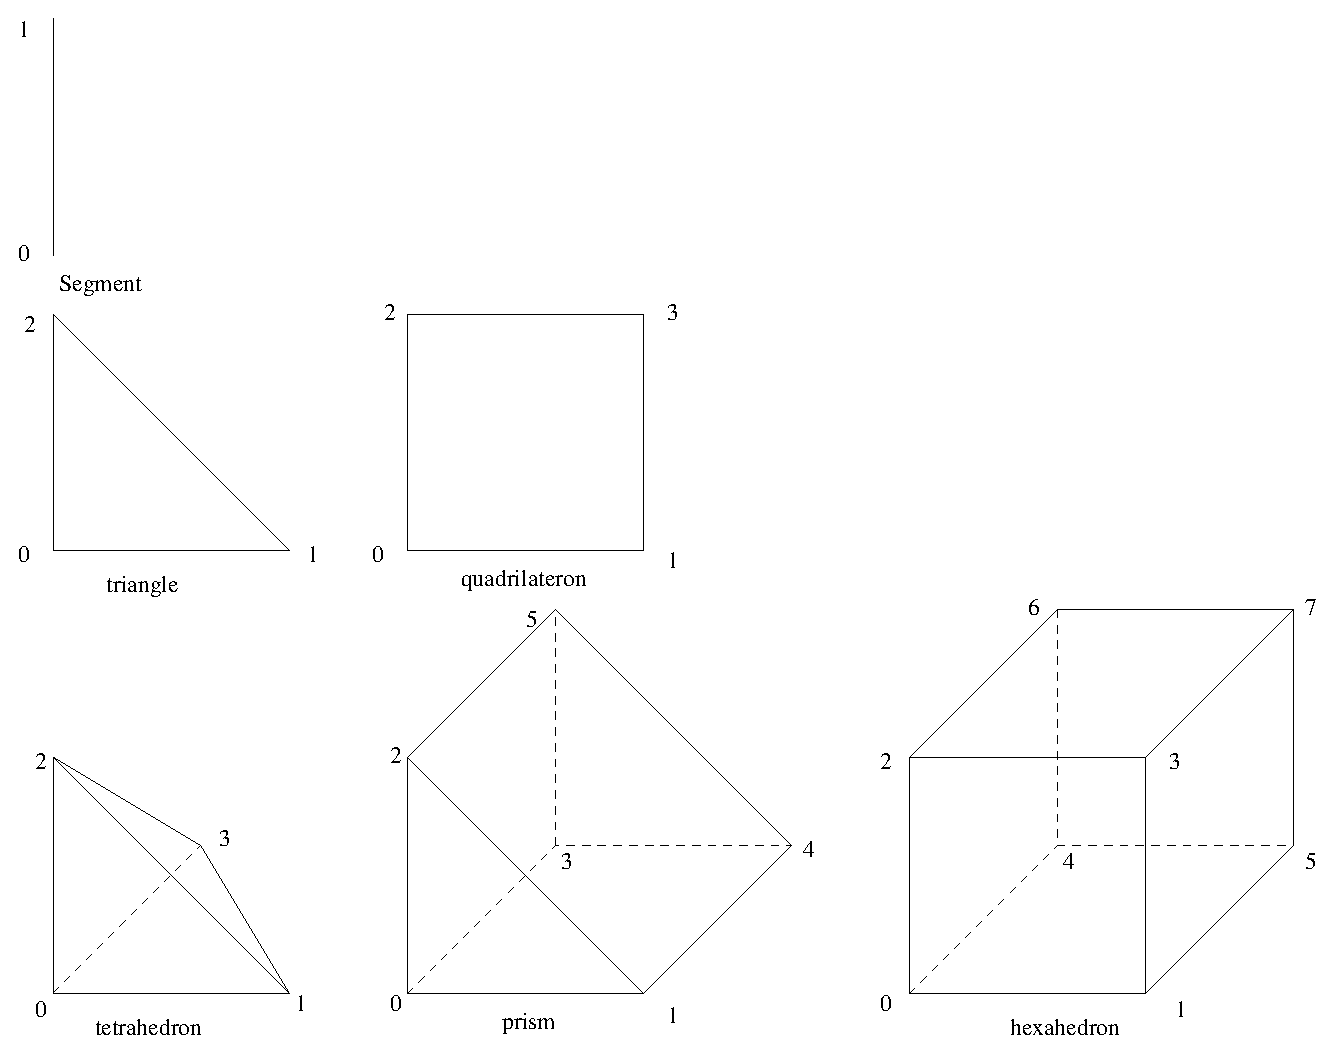
\includegraphics[width=15cm,angle=0]{getfemuser_elemf.eps}
  \end{center}
  \caption{ \it faces numerotation for usual elements }
\end{figure}

\subsection{Save, load and draw meshes}

In {\tt getfem\_mesh.h}, two methods are defined to load meshes from file and write meshes to a file. \\[0.5cm]
\begin{tabular}{|m{0.4\linewidth}|m{0.55\linewidth}|}\hline

  {\tt mesh.write\_to\_file(const std::string \&name)} & save the mesh into a file.\\ \hline

  {\tt mesh.read\_from\_file(const std::string \&name)} & load the mesh from a file.\\ \hline

\end{tabular} \\[0.5cm]
At this stage of development, the loading function only accepts to load classical elements (simplexes, prisms and parallelepipeds). If one needs other kind of elements, the loading function has to be extended.  \\[0.5cm]

A little tool allows to display a mesh using Gnuplot (and Perl). This tool is present in the directory {\tt contrib/} and of course you need to have a working distribution of Gnuplot installed on your system. This little tool is built when you execute a {\tt make} instruction on the root directory of GETFEM++. So, if GETFEM++ is normally installed on your system, you can change your current directory to {\tt contrib/} and execute the command \\[0.5cm]
{\tt draw\_mesh filename.mesh} \\[0.5cm]
where {\tt filename.mesh} is the file containing the mesh. This works only for meshes whose principal dimension is between 1 and 3. Examples of mesh files are also present into the directory {\tt contrib/} to test the program.

\subsection{example}

The following is an example of how to load a mesh and extract information on it. \\[0.5cm]
{\tt
  \#include <getfem\_mesh.h> \\
  \\
  getfem::getfem\_mesh mesh; \\
  \\
  int main(int argc, char *argv[]) \{ \\
    $\mbox{}\ \ $ try \{ \\
    $\mbox{}\ \ \ \ $ \\
    $\mbox{}\ \ \ \ $ // read the mesh from the file name given by the first argument \\
    $\mbox{}\ \ \ \ $ mesh.read\_from\_file(std::string(argv[0])); \\
    $\mbox{}\ \ \ \ $ \\
    $\mbox{}\ \ \ \ $ // List all the convexes\\
    $\mbox{}\ \ \ \ $ dal::bit\_vector nn = mesh.convex\_index(); \\
    $\mbox{}\ \ \ \ $ bgeot::size\_type i; \\
    $\mbox{}\ \ \ \ $ for (i << nn; i != bgeot::size\_type(-1); i << nn) \{\\
    $\mbox{}\ \ \ \ \ \ $ cout << "Convex of index " << i << endl; \\
    $\mbox{}\ \ \ \ \ \ $ bgeot::pconvex\_structure cvs =  mesh.structure\_of\_convex(i); \\
    $\mbox{}\ \ \ \ \ \ $ cout << "Number of vertices : " << cvs->nb\_points() << endl; \\
    $\mbox{}\ \ \ \ \ \ $ cout << "Number of faces : " << cvs->nb\_faces() << endl;\\
    $\mbox{}\ \ \ \ \ \ $ for (bgeot::size\_type f = 0; f < cvs->nb\_faces(); ++f) \{\\
    $\mbox{}\ \ \ \ \ \ \ \ $ cout << "face " << f << " has " << cvs->nb\_points\_of\_face(f); \\
    $\mbox{}\ \ \ \ \ \ \ \ $ cout << " vertices with local indexes : "; \\
    $\mbox{}\ \ \ \ \ \ \ \ $ for (bgeot::size\_type k = 0; k < cvs->nb\_points\_of\_face(f); ++k) \\
    $\mbox{}\ \ \ \ \ \ \ \ \ \ $ cout << cvs->ind\_points\_of\_face(f)[k] << " "; \\ 
    $\mbox{}\ \ \ \ \ \ \ \ $ cout << " and global indexes : ";\\
    $\mbox{}\ \ \ \ \ \ \ \ $ for (bgeot::size\_type k = 0; k < cvs->nb\_points\_of\_face(f); ++k) \\
    $\mbox{}\ \ \ \ \ \ \ \ \ \ $ cout << mesh.ind\_points\_of\_convex(i)(cvs->ind\_points\_of\_face(f)[k]) << " "; \\ 
    $\mbox{}\ \ \ \ \ \ \}$ \\
    $\mbox{}\ \ \ \ \}$ \\
    $\mbox{}\ \ $ \} DAL\_STANDARD\_CATCH\_ERROR; // catches standard errors\\
  \}

}

\section{Select finite element and integration methods}

In order to define a complete finite element procedure on a mesh, the structure {\tt getfem::mesh\_fem} is defined in the file {\tt getfem\_mesh\_fem.h}. Basically, this structure describe the finite element method on each element of the mesh, and can store information about boundary structure. It is possible to have an arbitrary number of finite element description for a single mesh. This is particularly necessary for mixed methods, but also to describe different data on the same mesh. One can instantiate a {\tt getfem::mesh\_fem} object as follows\\[0.5cm]
{\tt getfem::mesh\_fem mef(mesh); }\\[0.5cm]
where {\tt mesh} is an already existing mesh. The structure will be linked to this mesh and will react when modifications will be done on it. \\[0.5cm]
It is possible to specify element by element the finite element method, so that element of mixed types can be treated, even if the dimensions are different. For usual elements, the connection between two elements is done when the two elements are compatibles (same degrees of freedom on the common face). A numeration of the degrees of freedom is automatically done with a Cuthill Mc Kee like algorithm. You have to keep in mind that there is absolutely no connection between the numeration of vertices of the mesh and the numeration of the degrees of freedom. Every {\tt getfem::mesh\_fem} object has its own numeration. \\[0.5cm]
To select a particular finite element method on a given element, one can use \\[0.5cm]
{\tt mef.set\_finite\_element(i, ppf, ppi); }\\[0.5cm]
where {\tt i} is the index of the element, {\tt ppf} is the descriptor of the finite element method, and {\tt ppi} is the descriptor of the integration method. The list of all disponible descriptors of finite element methods is disponible in the file {\tt getfem\_fem.h}. A short description is also given in \cite{BAS_COMP}. The list of all disponible descriptors of integration methods is diponible in the file {\tt bgeot\_poly\_integration.h} for exact integration methods and in the file {\tt bgeot\_approx\_integration.h} for approximate integration methods.\\[0.5cm]
For instance if one needs to have a description of a $P_1$ finite element method on a triangle with an exact integration, the way set it is\\[0.5cm]
{\tt mef.set\_finite\_element(i, getfem::PK\_fem(2, 1), bgeot::simplex\_poly\_integration(2)); }\\[0.5cm]
where {\tt i} is still the index of the triangle. It is also possible to select a particular method directly on a set of element, paasing to {\tt mef.set\_finite\_element} a {\tt dal::bit\_vector} instead of a single index. For instance\\[0.5cm]
{\tt mef.set\_finite\_element(mesh.convex\_index(), getfem::PK\_fem(2, 1),\\$\mbox{}\ \ \ \ \ \ \ \ \ \ \ \ \ \ \ \ \ \ \ \ \ \ $ bgeot::simplex\_poly\_integration(2)); }\\[0.5cm]
select the method on all the element of the mesh.

Once a finite element method is defined on a mesh, it is possible to obtain information on it with the following methods (the list is not exhaustive).\\[0.5cm]
\begin{center} \begin{tabular}{|m{0.4\linewidth}|m{0.55\linewidth}|} \hline

  {\tt mef.convex\_index()} & Set of indexes (a {\tt dal::bit\_vector}) on which a finite element method is defined.  \\ \hline

  {\tt mef.linked\_mesh()} & gives a reference to the linked mesh.  \\ \hline

  {\tt mef.fem\_of\_element(i)} & gives a descriptor on the finite element method defined on element of index {\tt i}.  \\ \hline

  {\tt mef.int\_method\_of\_element(i)} & gives a descriptor on the integration method defined on element of index {\tt i}.  \\ \hline

  {\tt mef.nb\_dof\_of\_element(i)} & gives the number of degrees of freedom on the element of index {\tt i}.  \\ \hline

  {\tt mef.ind\_dof\_of\_element(i)} & gives a container (an array) with all the global indexes of the degrees of freedom of element of index {\tt i}.  \\ \hline

  {\tt mef.point\_of\_dof(i, j)} & gives a {\tt bgeot::base\_node} which represents the point associated with the dof of local index {\tt j} on element of index {\tt i}.  \\ \hline

  {\tt mef.point\_of\_dof(j)} & gives a {\tt bgeot::base\_node} which represents the point associated with the dof of global index {\tt j}.  \\ \hline

  {\tt mef.reference\_point\_of\_dof(i, j)} & gives a {\tt bgeot::base\_node} which represents the point associated with the dof of local index {\tt j} on element of index {\tt i} in the coordinates of the reference element.  \\ \hline

  {\tt mef.first\_convex\_of\_dof(j)} & gives the index of the first element on which the degree of freedom of global index {\tt j} is defined.  \\ \hline
  
  {\tt mef.nb\_dof()} & gives the total number of different degrees of freedom.  \\ \hline

  {\tt mef.clear()} & Clear the structure, no finite element method is still defined.  \\ \hline

  {\tt mef.add\_boundary\_elt(b, c, f)} & Add a face to a description of a boundary. Add the face {\tt f} of the element of index {\tt c} to the boundary of index {\tt b}.  \\ \hline
  
  {\tt mef.sup\_boundary\_elt(b, c, f)} & remove a face to a description of a boundary. remove the face {\tt f} of the element of index {\tt c} to the boundary of index {\tt b}.  \\ \hline
  
  {\tt mef.is\_convex\_on\_boundary(c, b)} & return wether or not the convex of index {\tt c}  has a face on the boundary of index {\tt b}.  \\ \hline
  
  {\tt mef.convex\_on\_boundary(b)} & return a {\tt dal::bit\_vector} containing all the indexes of all the elements having at least one face on boundary of index {\tt b}.  \\ \hline

  {\tt mef.faces\_of\_convex\_on\_boundary(c, b) } & return a {\tt dal::bit\_vector} containing all the local indexes of faces of the element of index {\tt c} which contained on the boundary of index {\tt b}.  \\ \hline

  {\tt mef.sup\_boundary(b) } & remove the boundary of index {\tt b}.  \\ \hline

\end{tabular} \end{center}


\section{Use standard assembling procedures}



\section{Compute arbitrary elementary matrices}

\section{incorporate new finite element methods in GETFEM++}

\section{Interpolate on different meshes}

\section{Compute $L^2$ and $H^1$ norms}

\section{Compute derivatives}

\section{Export and view a solution}

\section{Catch errors}

\section{Example : Laplacian program} (or own documentation ? )


\begin{thebibliography}{99}
% \bibliographystyle{apalike}
% \bibliographystyle{plain}
% \bibliography{all}
\bibitem{dh-to1984} 
  G. {\sc Dhatt, and  G. Touzot}
  {\it The Finite Element Method Displayed}, 
 J. Wiley \& Sons,  New York, 1984.
\bibitem{BAS_COMP}
  Y. {\sc Renard} (2002),
  {\it Elementary Computations in GETFEM++}.
\end{thebibliography}

\end{document}
